 
% An example of LaTeX use (uncomment, if you wish)
% %%% Ukázka použití některých konstrukcí LaTeXu

\subsection{Ukázka \LaTeX{}u}
\label{ssec:ukazka}

This short subsection serves as an~example of basic \LaTeX{} constructs,
which can be useful for writing a~thesis.

Let us start with lists:

\begin{itemize}
\item The logo of Matfyz is displayed in figure~\ref{fig:mff}.
\item This is subsection~\ref{ssec:ukazka}.
\item Citing literature~\cite{lamport94}.
\end{itemize}

Different kinds of dashes:
red-black (short),
pages 16--22 (middle),
$45-44$ (minus),
and this is --- as you could have expected --- a~sentence-level dash,
which is the longest.
(Note that we have follwed \verb|a| by a~tilde instead of a~space
to avoid line breaks at that place.)

\newtheorem{theorem}{Theorem}
\newtheorem*{define}{Definition}	% Definice nečíslujeme, proto "*"

\begin{define}
A~{\sl Tree} is a connected graph with no cycles.
\end{define}

\begin{theorem}
This theorem is false.
\end{theorem}

\begin{proof}
False theorems do not have proofs.
\end{proof}

\begin{figure}
	\centering
	
\includegraphics[width=30mm]{../img/logo.eps}
	\caption{Logo of MFF UK}
	\label{fig:mff}
\end{figure}


\chapter*{Conclusion}
\addcontentsline{toc}{chapter}{Conclusion}
Based on the experiments it can be said, that the framework works fine and it can be successfully used to speed up computation in the local network. Although the achieved speed up does not grow linearly with the increasing number of nodes, it can be quite significant. It was not tested in WAN environments, however, according to the results, the transfers of the data takes indispensable portion of the whole processing time, so the improvement depends on the network throughput. 

As is being discussed in \hyperref[Problems-alternatives-and-possible-improvements]{chapter 4}, the framework could be further improved. To achieve more effective distribution of the work, more sophisticated scheduling could be employed. Also it was shown, that some redundancy for prevention of re-computing whole node could be useful. Because of the speed of the network the data transfers generally seems to be a bottleneck, so good scheduling algorithm appears to be very important, together with optimal choice of the chunk size. This leads us to a conclusion, that in reliable network environments is probably better idea to centralize logic to special node in order to achieve better performance and accept potential malfunctions caused by the control node failure.

\chapter*{Appendix A - Installation and use}
\section{Download} 
First it's essential to get the source code. You can clone the code directly from the git repository using command
\begin{verbatim}
# git clone https://github.com/vojtsek/VideoCompression.git
\end{verbatim}
Alternatively you can download the zip file and unpack it in some directory.

\section{Requirements, installation and first run}
To run the program successfully it's essential to have \textit{ffmpeg} and \textit{ffprobe} installed on your computer. Although technically it doesn't matter which codec is used, the program currently uses only H.264 standard for encoding of the output, so it assumes the \textit{ffmpeg} has been compiled with the \textit{x264} codec. Otherwise the program does not have any special requirements except standard libraries which should be available on all UNIX systems, so once you installed these programs, you can change to the directory containing the source code and run the installation script:
\begin{verbatim}
# cd DVC
# ./install.sh
\end{verbatim}
The installation script is a regular Bash script, so the Bourne again shell interpreter is required to run it successfully. It explores your computer, i.e. gets the IP address, finds location of \textit{ffmpeg} binaries etc. Then it creates home directory for the program. The home directory contains data of the program's run. These include intermediate results as well as the final result and log files. The installation continues with generating the configuration file. This file is crucial for the framework. Before setting each option, the script prompts you for confirmation of the value. If you type nothing and just press the Enter key, the suggested value is used, otherwise the script uses your input. The resulting file is stored in the \textit{bin} directory which is created during the installation. It's a plain text file so you can edit it anytime in the future. The script then continues with compilation of the program. If everything is all right, you can change to the newly created \textit{bin} directory and continue. The directory \textit{bin/lists} contains some supporting files that should not be change, otherwise the program could behave improperly.

The last step before you can run the program is to check the configuration. The configuration is saved in the \textit{bin/CONF} file, which is created by the installation script. It's important to provide valid path to the \textit{ffmpeg} and \textit{ffprobe} executable and address with port of the neighbor that should be contacted initially. Otherwise you won't be able to join the network. The field \textit{MY\_IP} is not essential as long as the initial neighbor is alive - it will be recognized automatically. 

Then you can finally run the program. Some of the settings can be changed by providing options, the available ones are listed in the table 4.1.

\begin{table}[h]
\begin{center}
 \begin{tabular}{ | l | c |}
   \hline
-s & no address will be contacted initially \\ \hline
-n [address]:port\_number & node to contact initially \\ \hline
-a [address]:port\_number & address and port to bound to \\ \hline
-h & directory path to the home directory \\ \hline
-i file & file to encode \\ \hline
-p port & listening port \\ \hline
-d level & debug level \\ \hline
-q quality & quality of encoding \\ \hline
 \end{tabular}
 \caption{Table of the possible options.}
 \end{center}
\end{table}

If the string "\textit{IPv4}" appears among parameters, the program will use only the IPv4 addresses\footnote{https://en.wikipedia.org/wiki/IPv4},
in which case should be the \textit{CONF} file changed appropriately.

\section{Using the program}
When you run the program, the initial screen appears. You can choose desired action then using function keys. You can see the initial screen in the figure 4.1. Available options are highlighted.
\begin{figure}[h]
\begin{center}
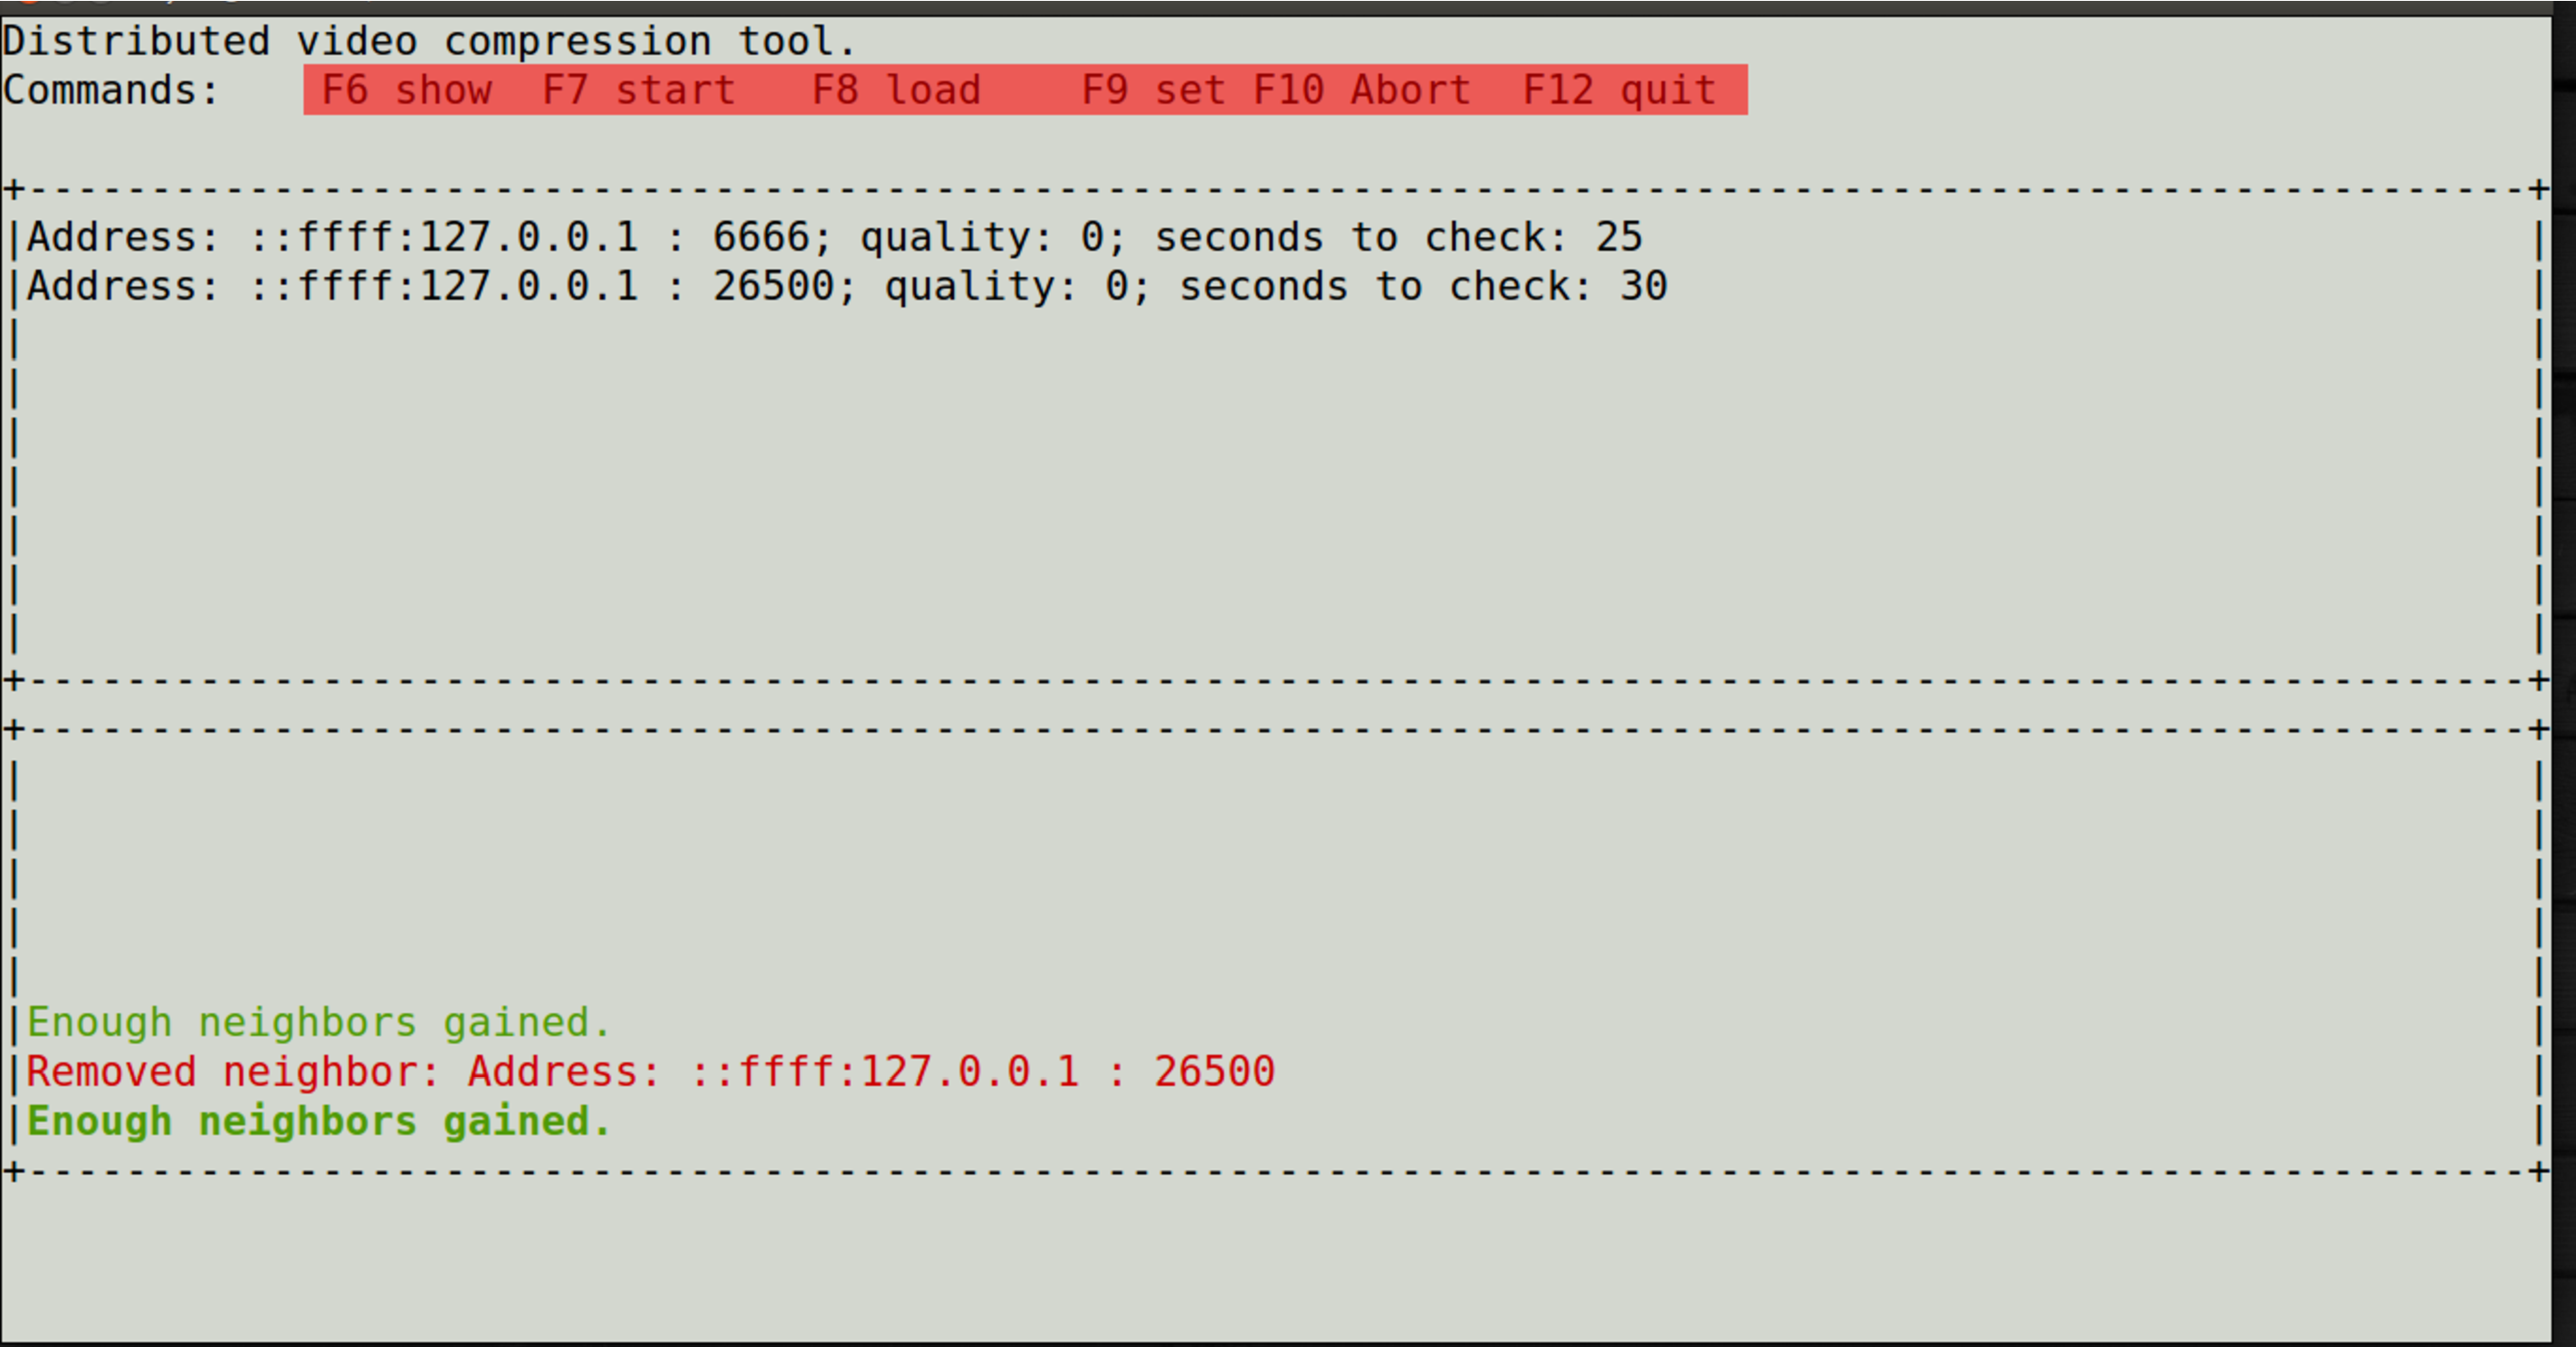
\includegraphics[scale=0.35]{./img/init-screen.pdf}
\label{initial-screen}
\caption[initial-screen]{Initial screen after joining.}
\end{center}
\end{figure}

The important key bindings are listed in the table 4.2.
\begin{table}[h]
\begin{center}
 \begin{tabular}{ | l | c |}
   \hline
   F6 & Show information \\ \hline
   F7 & Start the process \\ \hline
   F8 & Load the file \\ \hline
   F9 & Set values \\ \hline
   F10 & Abort the process \\ \hline
   F12 & Quit the program \\ \hline
   Up, Down & Traverse available options \\ \hline
   Enter & Confirm the input \\
 	\hline
 \end{tabular}
 \caption{Table of the control keys.}
 \end{center}
\end{table}

First you should load the video file. When the corresponding function key is pressed, the program prompts you for the file location. You can type in the absolute path of the file. Once you use the file, it is stored in history which you can browse using up and down arrow keys. This can be seen in the figure 4.2.
\begin{figure}[h]
\begin{center}
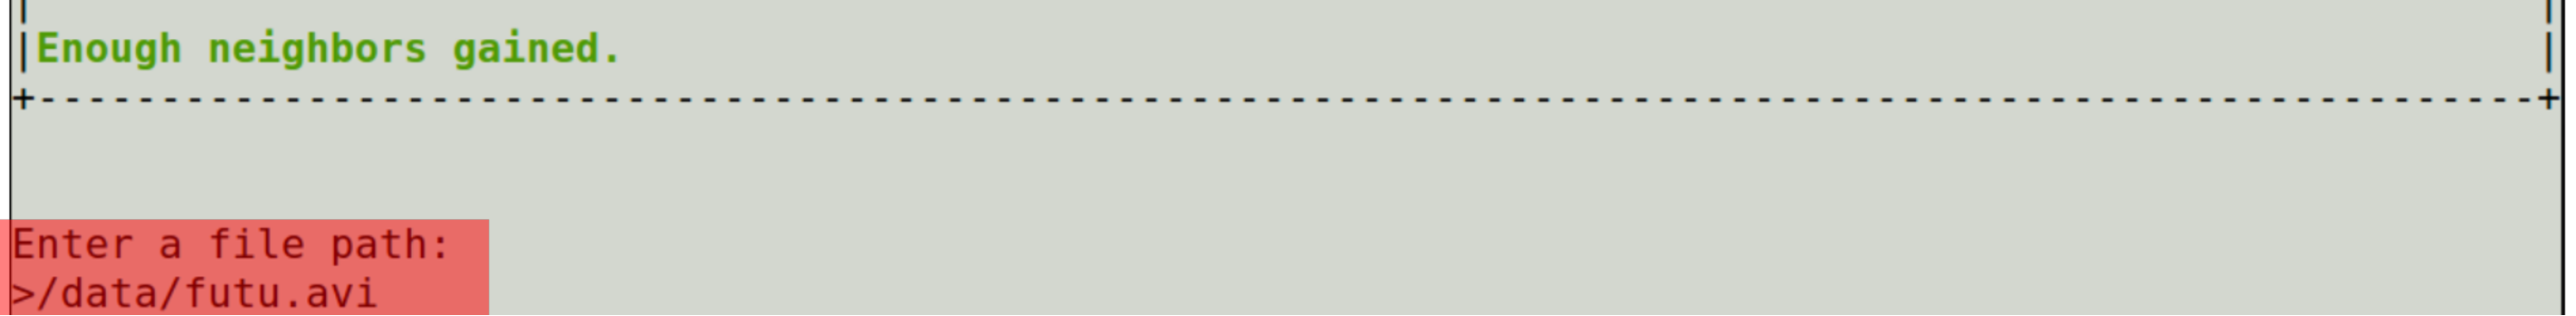
\includegraphics[scale=0.35]{./img/loading.pdf}
\label{loading-files}
\caption{Loading the file.}
\end{center}
\end{figure}

Then you can set some parameters or show different information using F6 respectively F9 function keys. These keys provides set of options which you can choose from. When you are satisfied with the settings, you can start the process.
The program then starts splitting the file and distributing the chunks while informing you about the progress. When the process is done, the file is joined and you can do further actions. Some screenshots from the ongoing process are displayed at the figures 4.3, 4.4 and 4.5
\begin{figure}[h]
\begin{center}
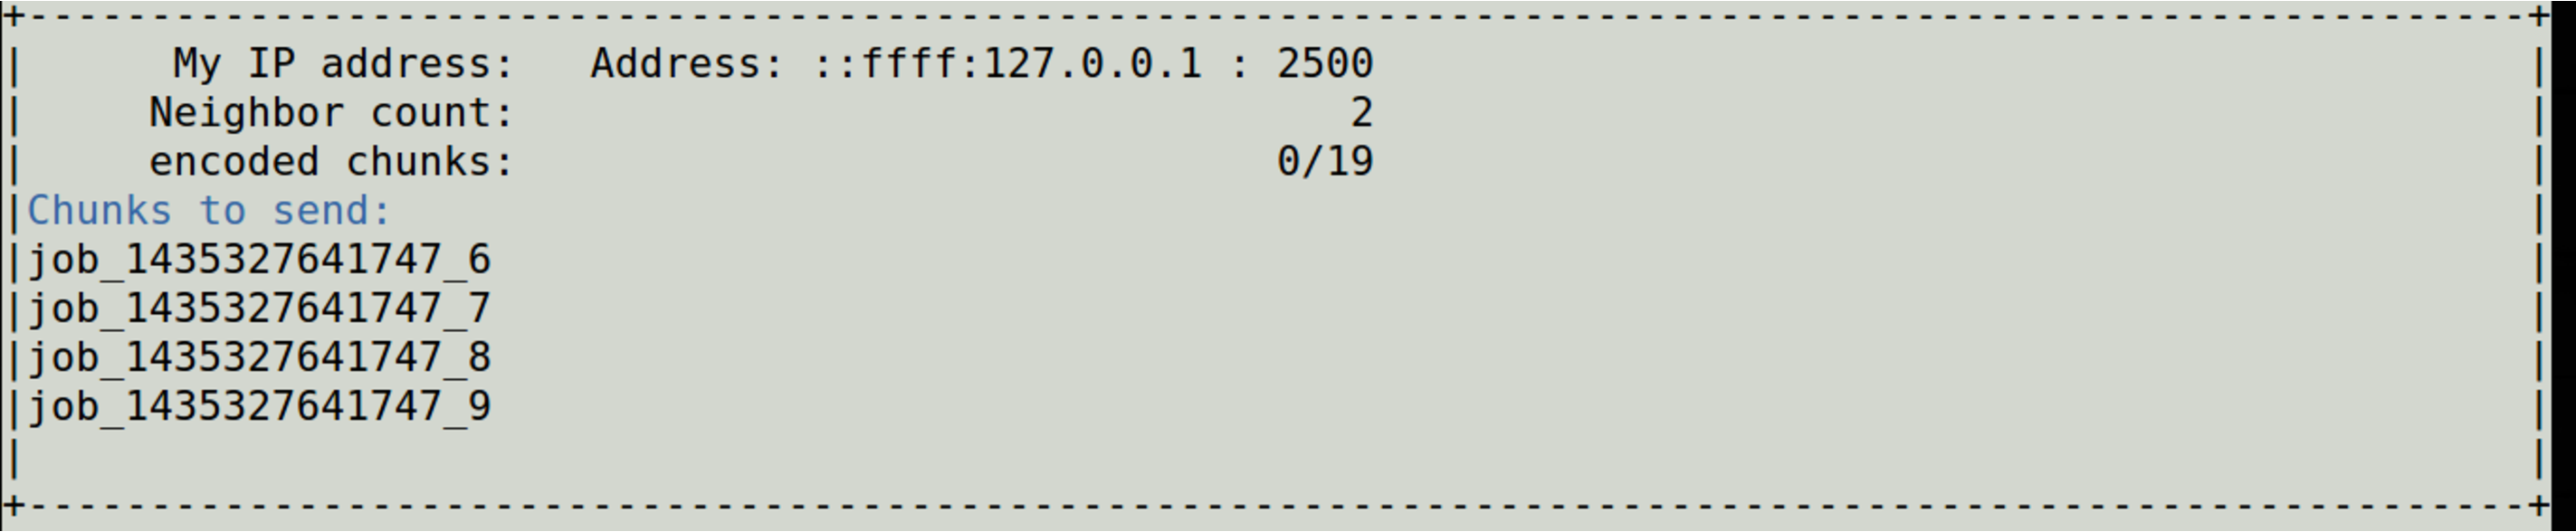
\includegraphics[scale=0.35]{./img/process-initiator.pdf}
\caption{Overview of the process.}
\end{center}
\end{figure}
\begin{figure}[h]
\begin{center}
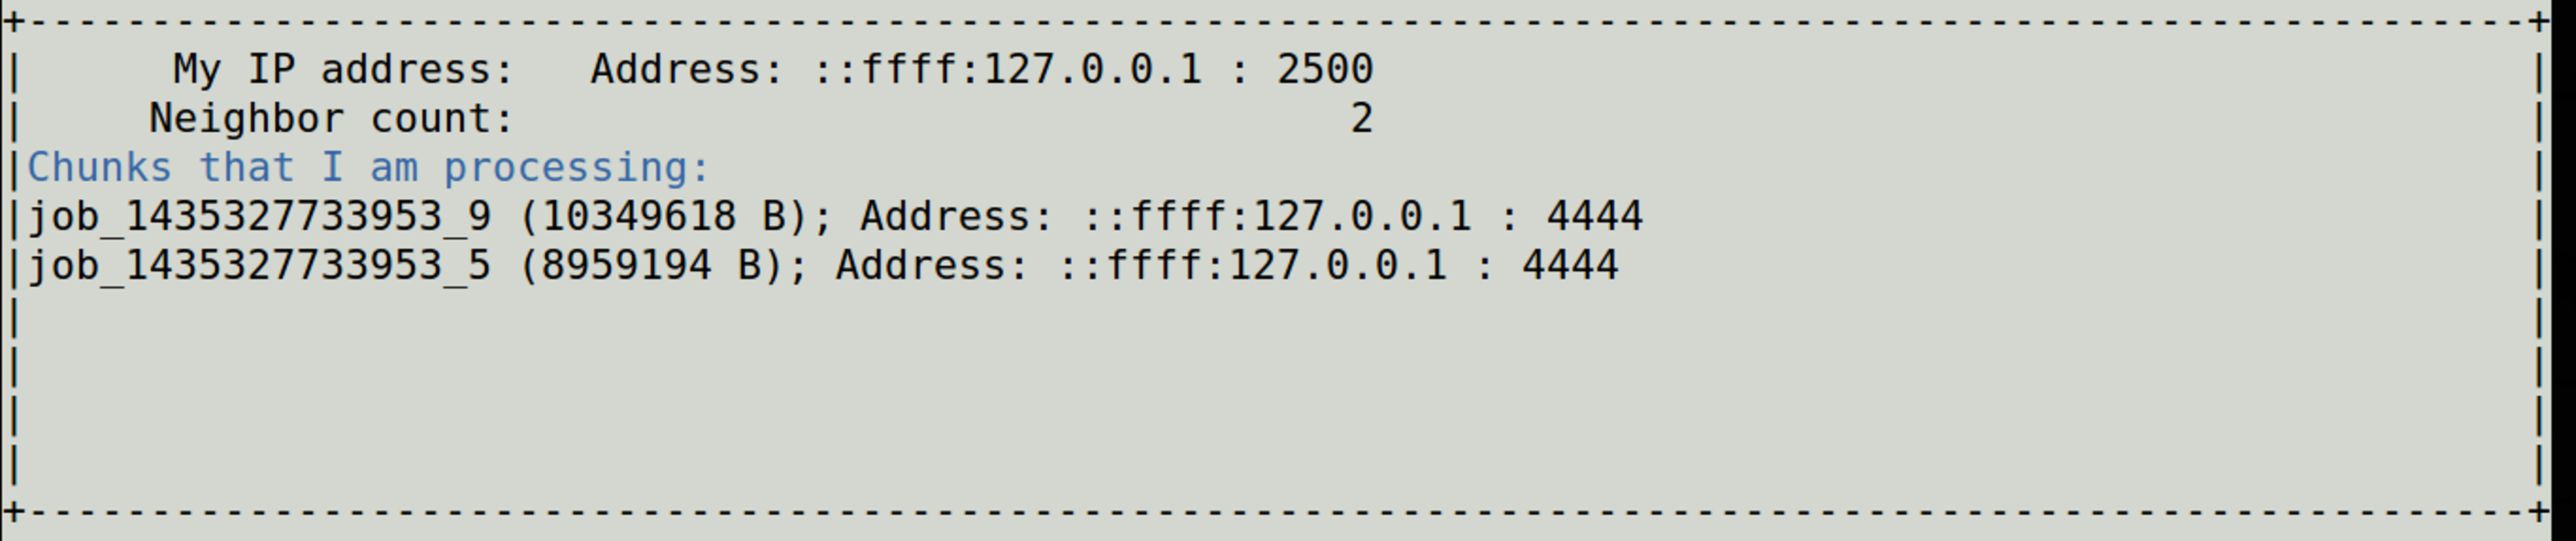
\includegraphics[scale=0.35]{./img/processing.pdf}
\caption{Processing of the tasks.}
\end{center}
\end{figure}
\begin{figure}[h]
\begin{center}
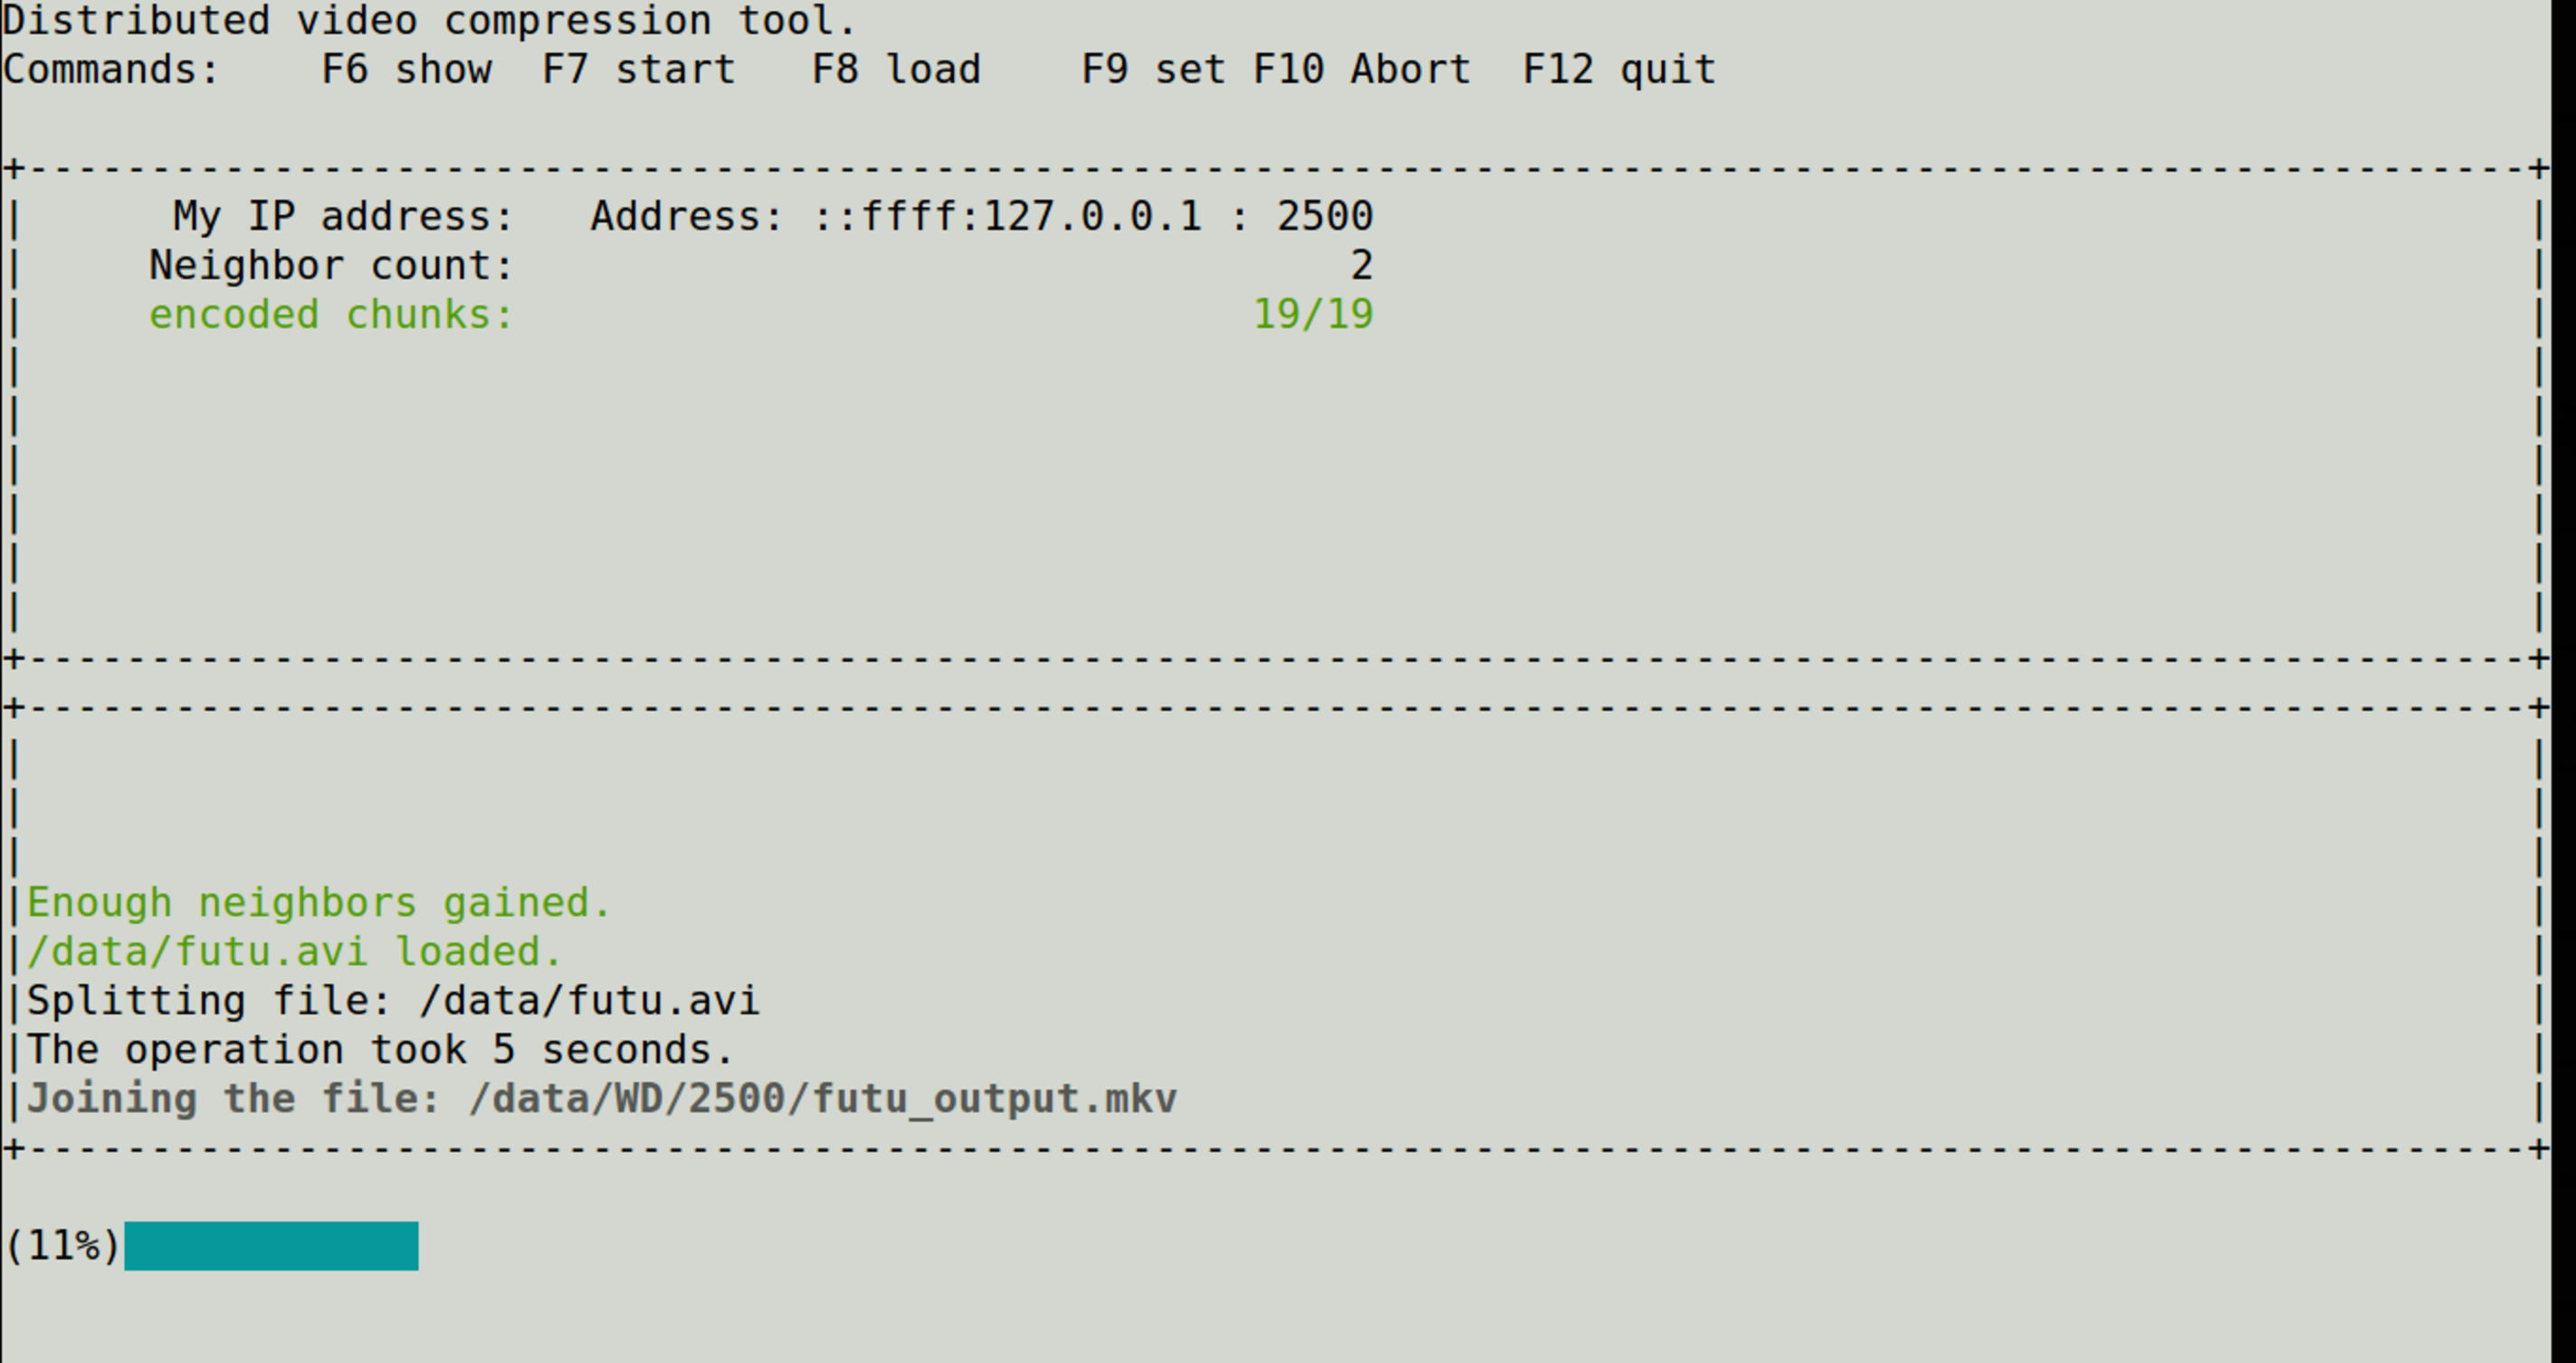
\includegraphics[scale=0.35]{./img/joining.pdf}
\caption{Joining the file.}
\end{center}
\end{figure}

To obtain more information about what is going on, the \textit{-d} option may be used which allows to specify level of debug messages that will be shown.

%%% Bibliography
\bibliographystyle{csplainnat}
\bibliography{literature}
\addcontentsline{toc}{chapter}{\bibname}

%%% Figures used in the thesis (consider if this is needed)
\listoffigures

%%% Tables used in the thesis (consider if this is needed)
\listoftables

%%% Abbreviations used in the thesis, if any, including their explanation
\chapwithtoc{List of Abbreviations}
\begin{itemize}
\item \textbf{LAN} Local Area Network
\item \textbf{TCP} Transmission control protocol
\item \textbf{IPv4 (IPv6)} Internet Protocol version 4 (version 6)
\item \textbf{API} Application programming interface
\item \textbf{GUI} Graphical User Interface
\item \textbf{HTML} Hypertext Markup Language
\item \textbf{OS} Operating System
\item \textbf{STL} Standard Template Library
\item \textbf{JSON} JavaScript Object Notation
\item \textbf{MTU} Maximum Transmission Unit
\item \textbf{B, kB, MB, GB} Byte, kiloByte, megaByte, gigaByte
\end{itemize}

%%% Attachments to the bachelor thesis, if any (various additions such
%%% as programme extracts, diagrams, etc.). Each attachment must be referred to
%%% at least once from one's own text of the thesis. Attachments are numbered.
\chapwithtoc{Attachments}

\section*{Appendix A - Installation and use}
\subsection*{Download} 
First it's essential to get the source code. You can clone the code directly from the git repository using command
\begin{verbatim}
# git clone https://github.com/vojtsek/VideoCompression.git
\end{verbatim}
Alternatively you can download the zip file and unpack it in some directory.

\subsection*{Requirements, installation and first run}
You must have \textit{ffmpeg} and \textit{ffprobe} installed on your computer, if you want to run the program successfully. Although technically it doesn't matter which codec is used, the program currently uses H.264 standard as a default, so it assumes the \textit{ffmpeg} has been compiled with the \textit{x264} codec support. Otherwise the program does not have any special requirements except standard libraries which should be available on all UNIX systems. When you install these programs, you can change to the directory containing the source code and run the installation script:
\begin{verbatim}
# cd VideoCompression
# ./install.sh
\end{verbatim}
The installation script is a regular Bash script, so the Bourne again shell interpreter is required to run it successfully. It uses utilities that are common part of every Linux distribution. If some of it is not present, you can either install it or do the preparation yourself. The script explores your computer, i.e. gets the IP address, finds location of \textit{ffmpeg} binaries etc. Then it creates home directory for the program. The home directory contains data of the program's run. These include intermediate results as well as the final result and log files. The installation continues with generating the configuration file. This file is crucial for the framework. Before setting each option, the script prompts you for confirmation of the value. If you type nothing and just press the \textit{Enter} key, the suggested value is used, otherwise the script uses your input. The result configuration file is stored in the \textit{bin/} directory which is created during the installation. It's a plain text file so you can edit it anytime in the future. The script then continues with compilation of the program. If everything is all right, you can change to the newly created \textit{bin/} directory and continue. The directory \textit{bin/lists/} contains some supporting files that should not be changed. Otherwise the program could behave improperly.

The last step before you can run the program is to check the configuration. The configuration is saved in the \textit{bin/CONF} file, which is created by the installation script. It's important to provide valid path to the \textit{ffmpeg} and \textit{ffprobe} executables and address with port of the neighbor that should be contacted initially. Otherwise you won't be able to join the network. The field \textit{MY\_IP} is not essential as long as the initial neighbor is alive - it will be recognized automatically. 

Then you can finally run the program. Some of the settings can be changed by providing options, the available ones are listed in the table 4.1.

\begin{table}[h]
\begin{center}
 \begin{tabular}{ | l | c |}
   \hline
-s & no address will be contacted initially \\ \hline
-n [address]:port\_number & node to contact initially \\ \hline
-a [address]:port\_number & address and port to bound to \\ \hline
-h & directory path to the home directory \\ \hline
-i file & file to encode \\ \hline
-p port\_number & listening port \\ \hline
-d level & debug level \\ \hline
-q quality & quality of encoding \\ \hline
 \end{tabular}
 \caption{Table of the possible options.}
 \end{center}
\end{table}

If the string \textit{IPv4} appears among parameters, the program will use only the IPv4 addresses\footnote{https://en.wikipedia.org/wiki/IPv4},
in which case should be the \textit{CONF} file changed appropriately.

\subsection*{Using the program}
When you run the program, the initial screen appears. You can perform desired action using function keys. You can see the initial screen in the Figure 4.1. Available options are highlighted.
\begin{figure}[h]
\begin{center}
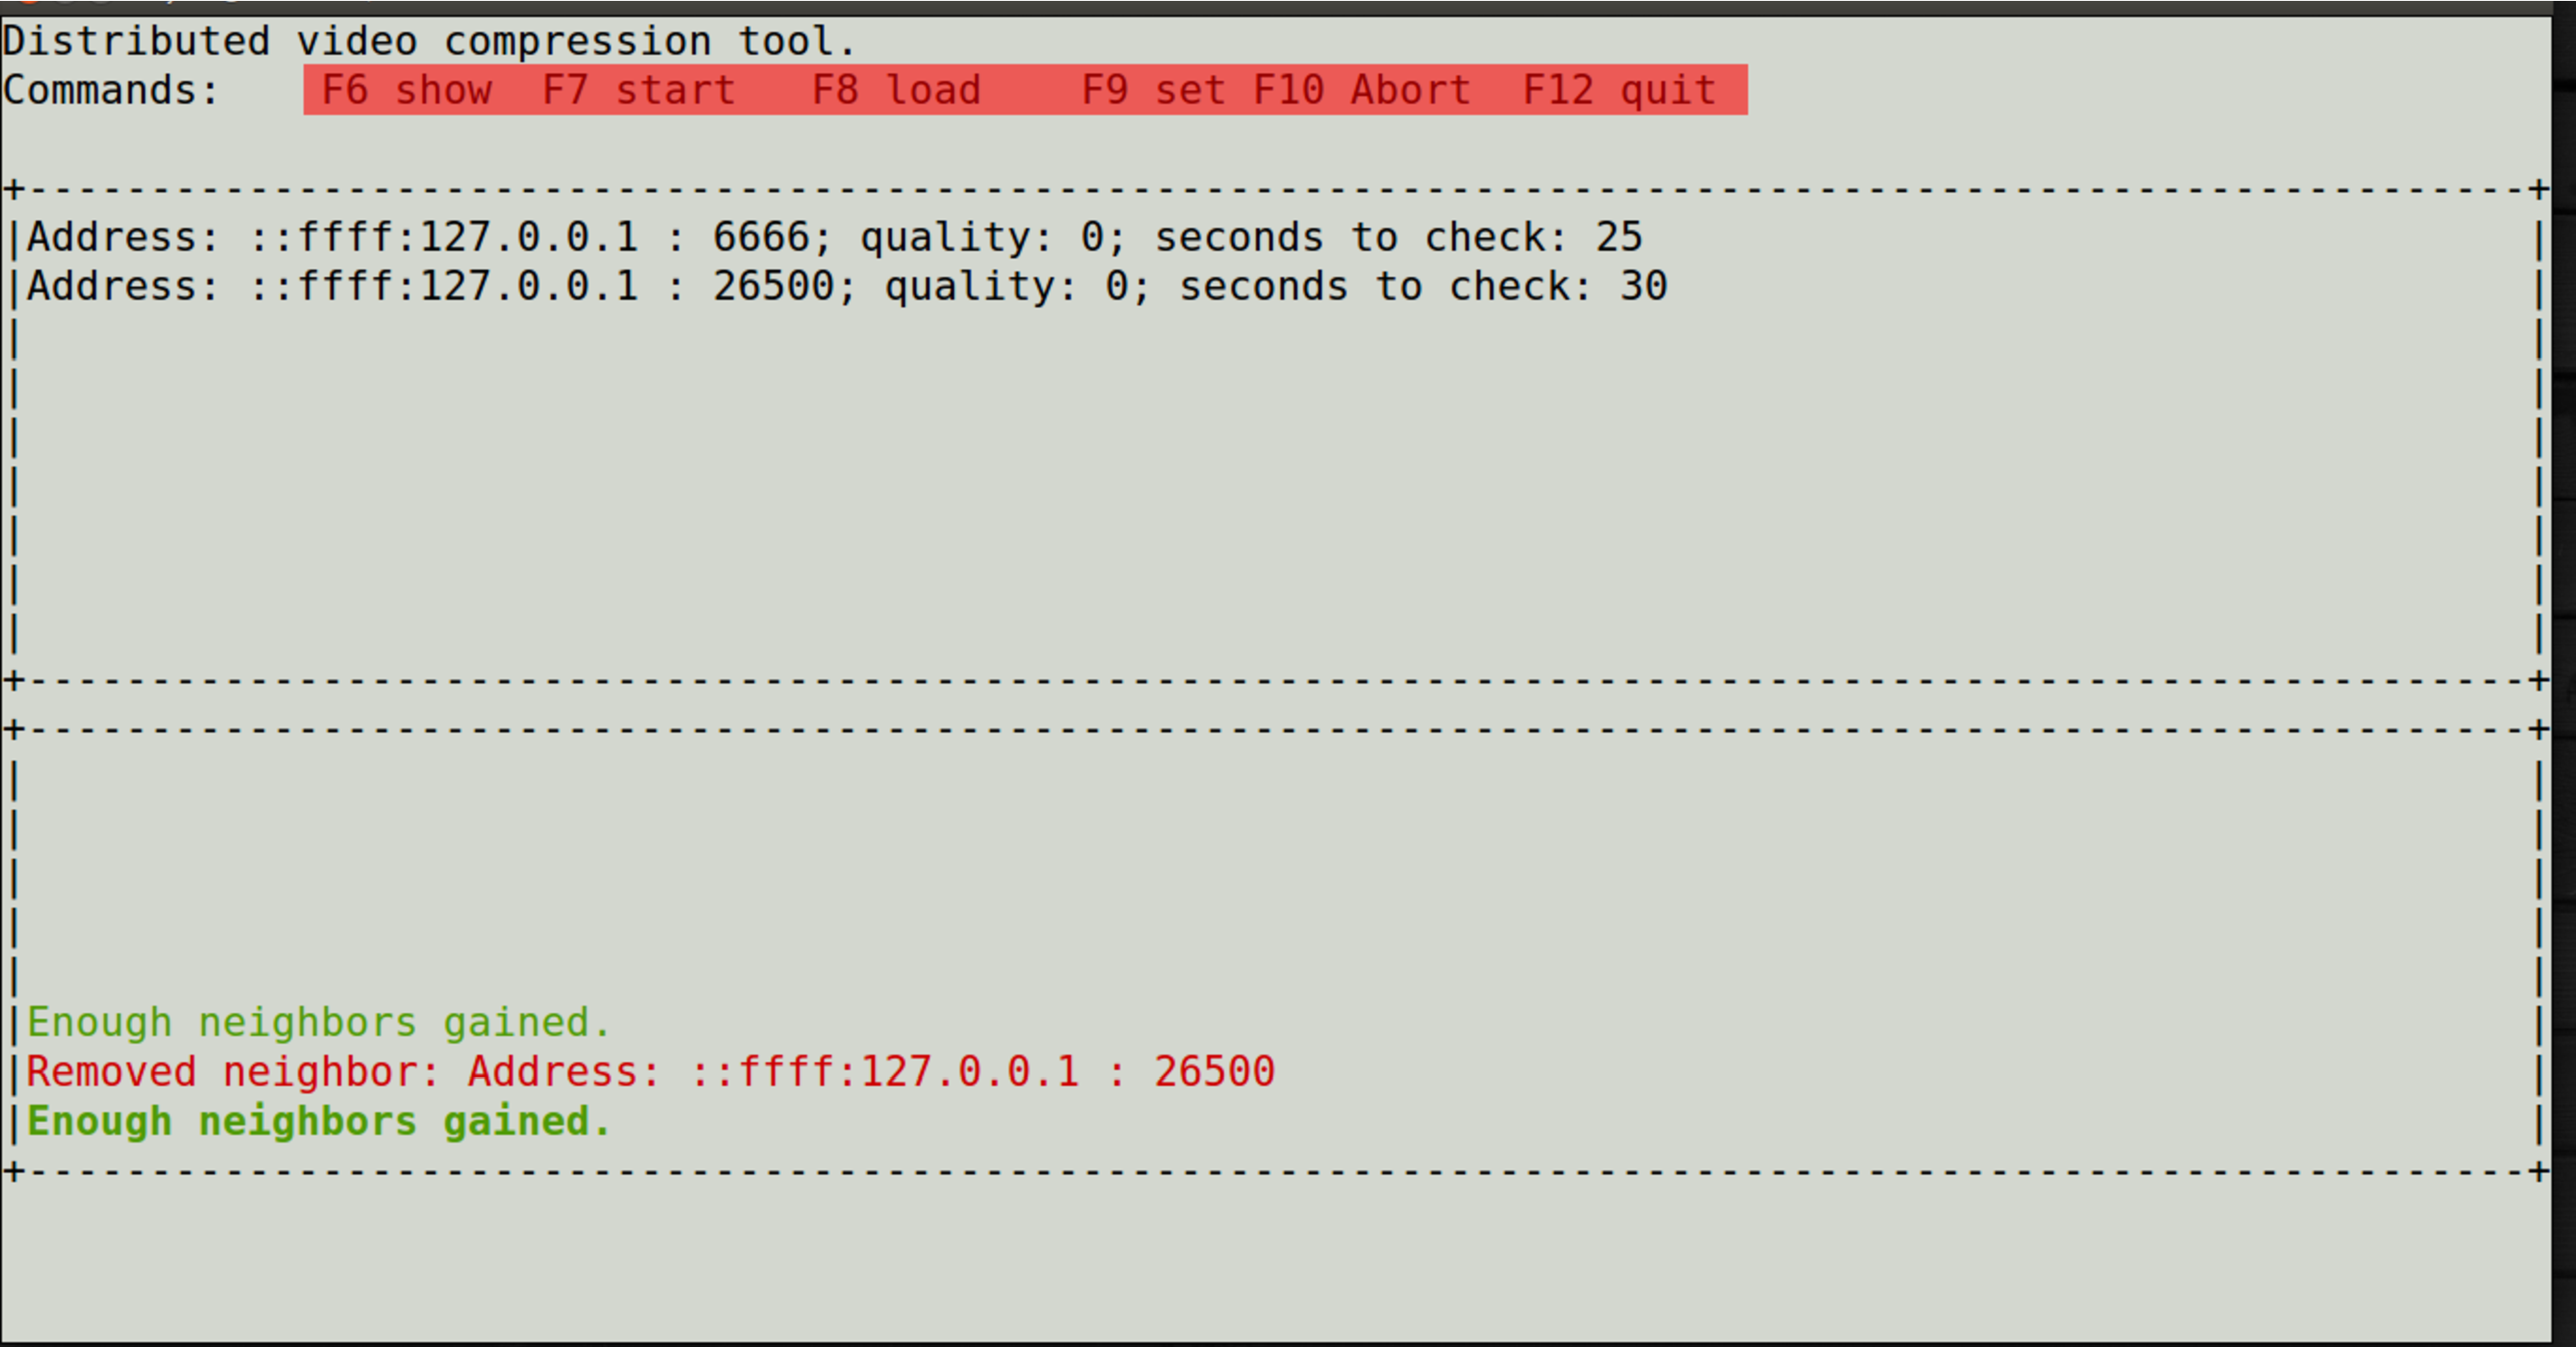
\includegraphics[scale=0.30]{./img/init-screen.pdf}
\label{initial-screen}
\caption[initial-screen]{Initial screen after joining.}
\end{center}
\end{figure}

The important key bindings are listed in the table 4.2.
\begin{table}[h]
\begin{center}
 \begin{tabular}{ | l | c |}
   \hline
   F6 & Show information \\ \hline
   F7 & Start the process \\ \hline
   F8 & Load the file \\ \hline
   F9 & Set values \\ \hline
   F10 & Abort the process \\ \hline
   F12 & Quit the program \\ \hline
   Up, Down & Traverse available options \\ \hline
   Enter & Confirm the input \\
 	\hline
 \end{tabular}
 \caption{Table of the control keys.}
 \end{center}
\end{table}

First you should load the video file. When the corresponding function key is pressed, the program prompts you for the file location. You can type in the absolute path of the file. Once you use the file, it is stored in history which you can browse using up and down arrow keys. This can be seen in the Figure 4.2.
\begin{figure}[h]
\begin{center}
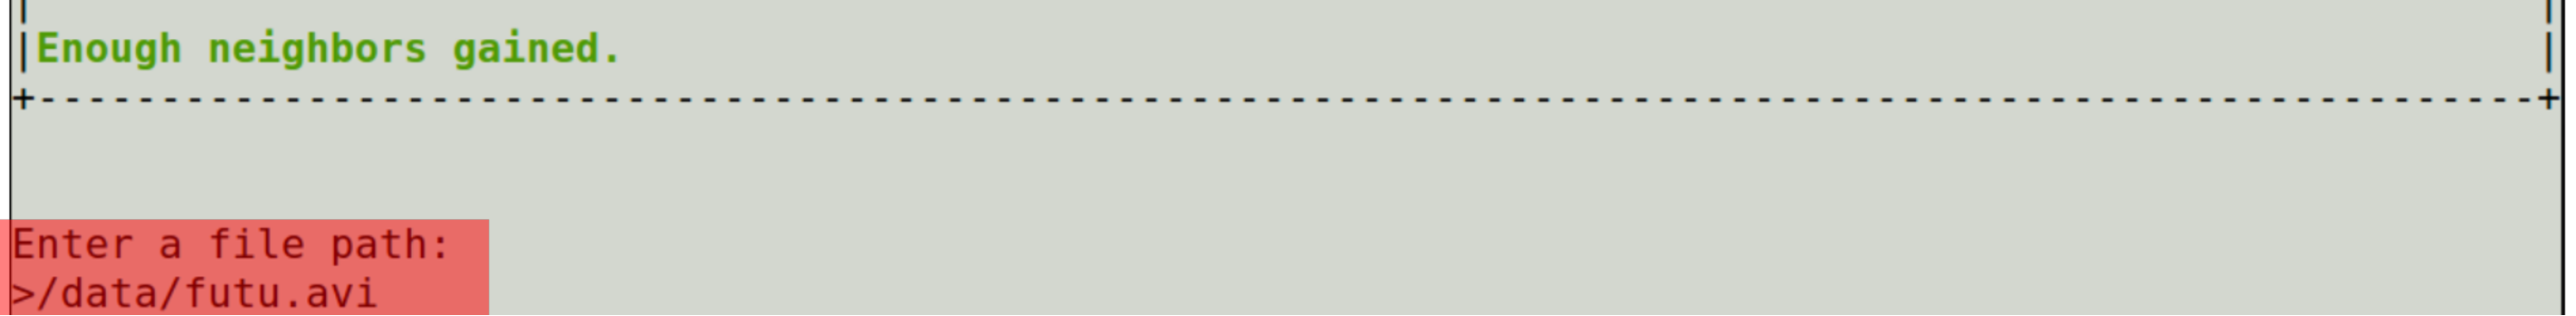
\includegraphics[scale=0.30]{./img/loading.pdf}
\caption{Loading the file.}
\end{center}
\end{figure}

Then you can set some parameters or show different information using F6 respectively F9 function keys. These keys provides set of options which you can choose from. When you are satisfied with the settings, you can start the process.
The program then starts splitting the file and distributing the chunks. It also keeps informing you about the progress. When the process is done, the file is joined and you can do further actions. You can find the result in the provided work directory. There should appear new folder with a timestamp of the current job. It contains the file named \textit{orig\_output.mkv}, where \textit{orig} is the base name of the input file. Some screenshots from the ongoing process are displayed in the Figures 4.3, 4.4 and 4.5
\begin{figure}[h]
\begin{center}
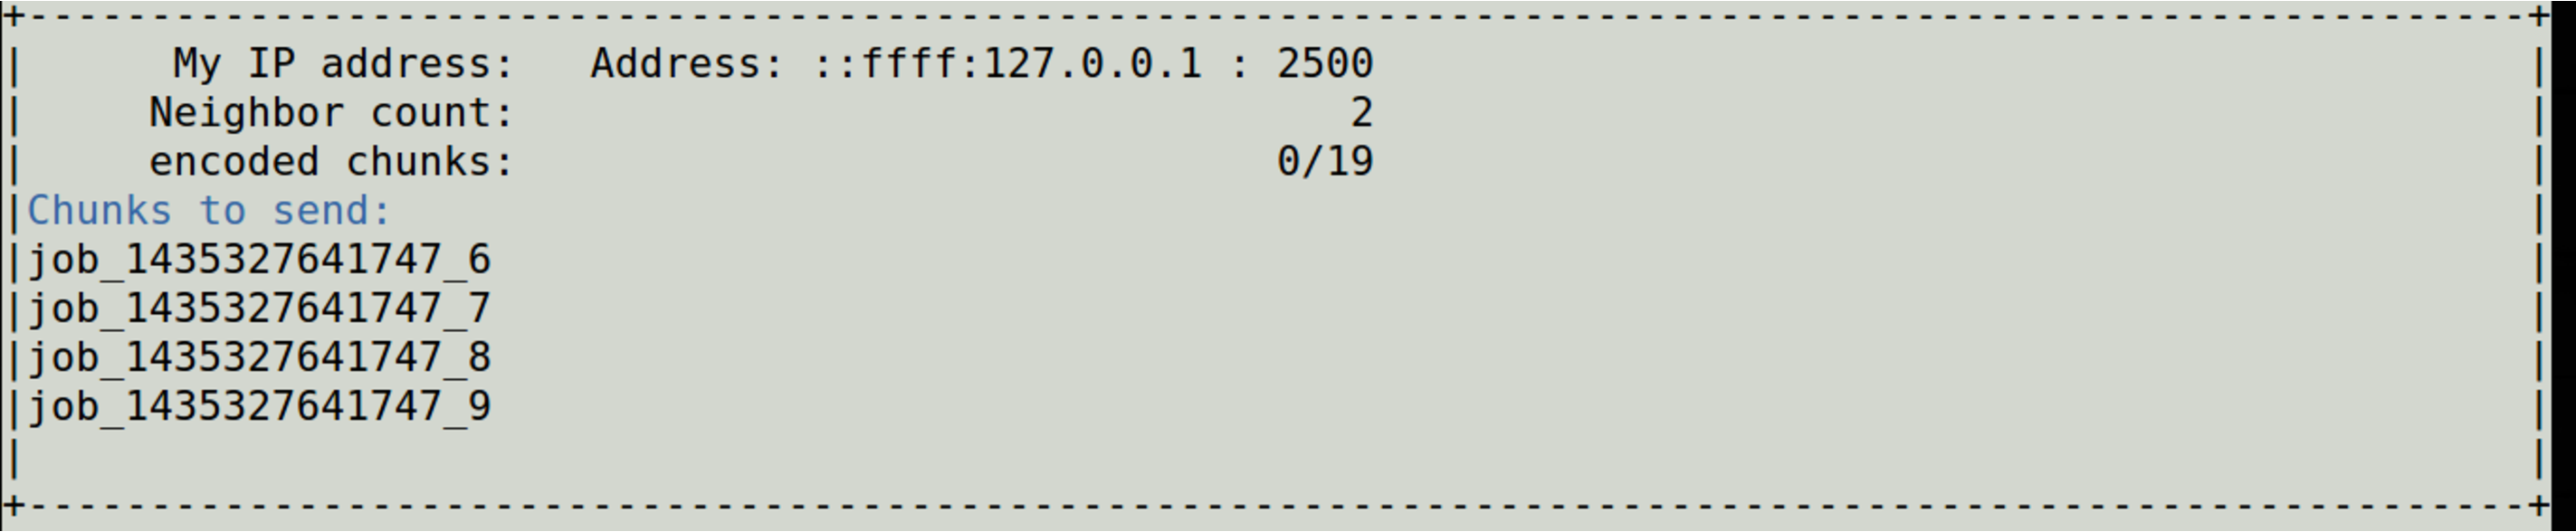
\includegraphics[scale=0.30]{./img/process-initiator.pdf}
\caption{Overview of the process.}
\end{center}
\end{figure}
\begin{figure}[h]
\begin{center}
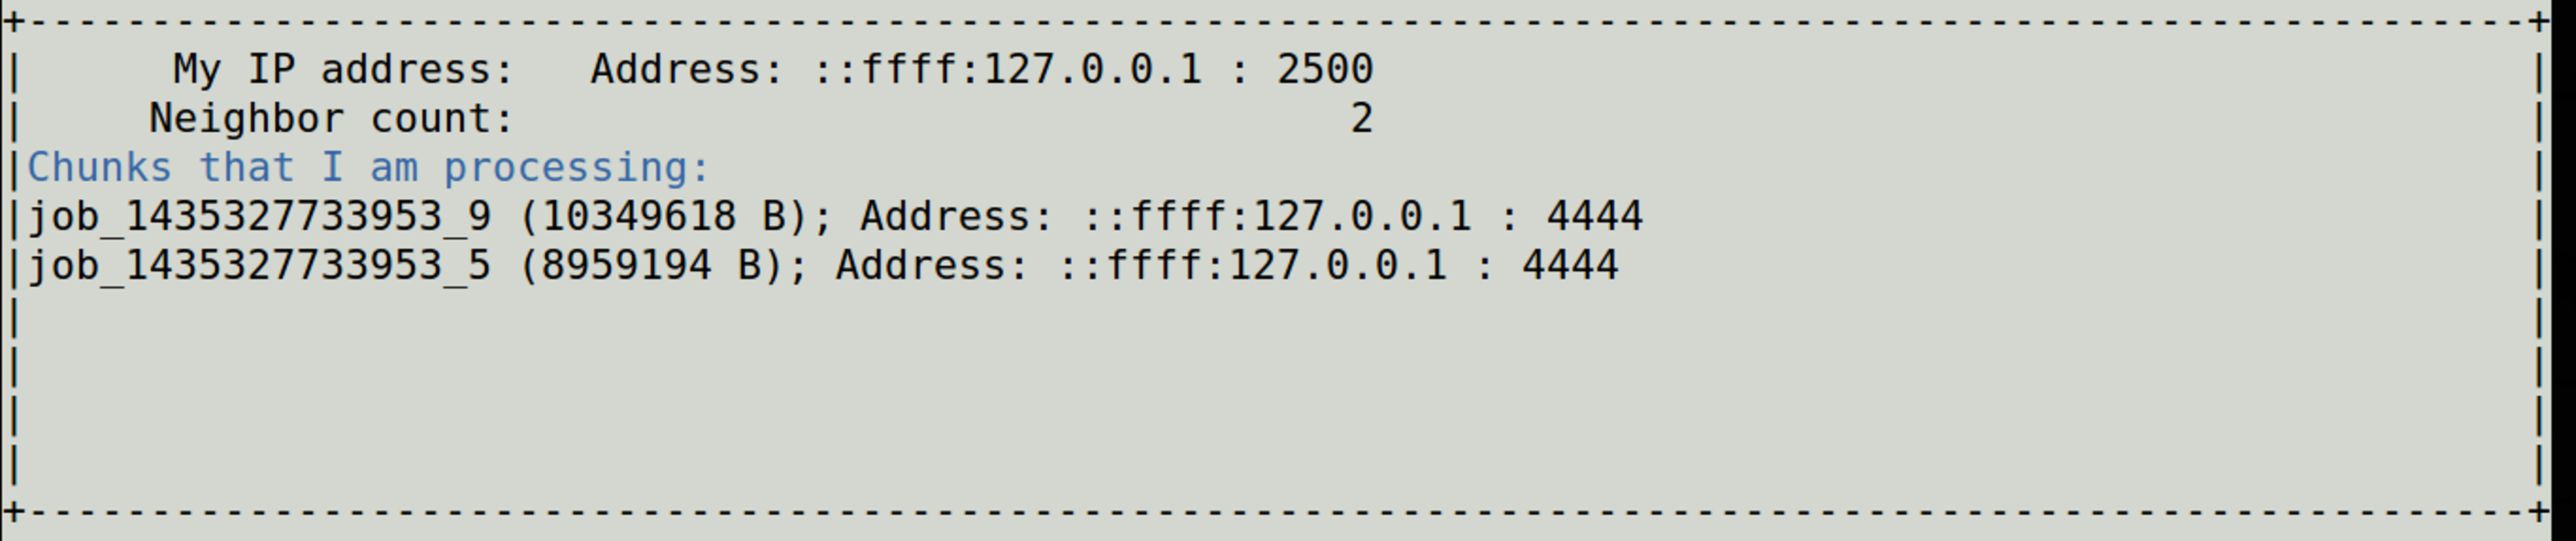
\includegraphics[scale=0.30]{./img/processing.pdf}
\caption{Processing of the tasks.}
\end{center}
\end{figure}
\begin{figure}[h]
\begin{center}
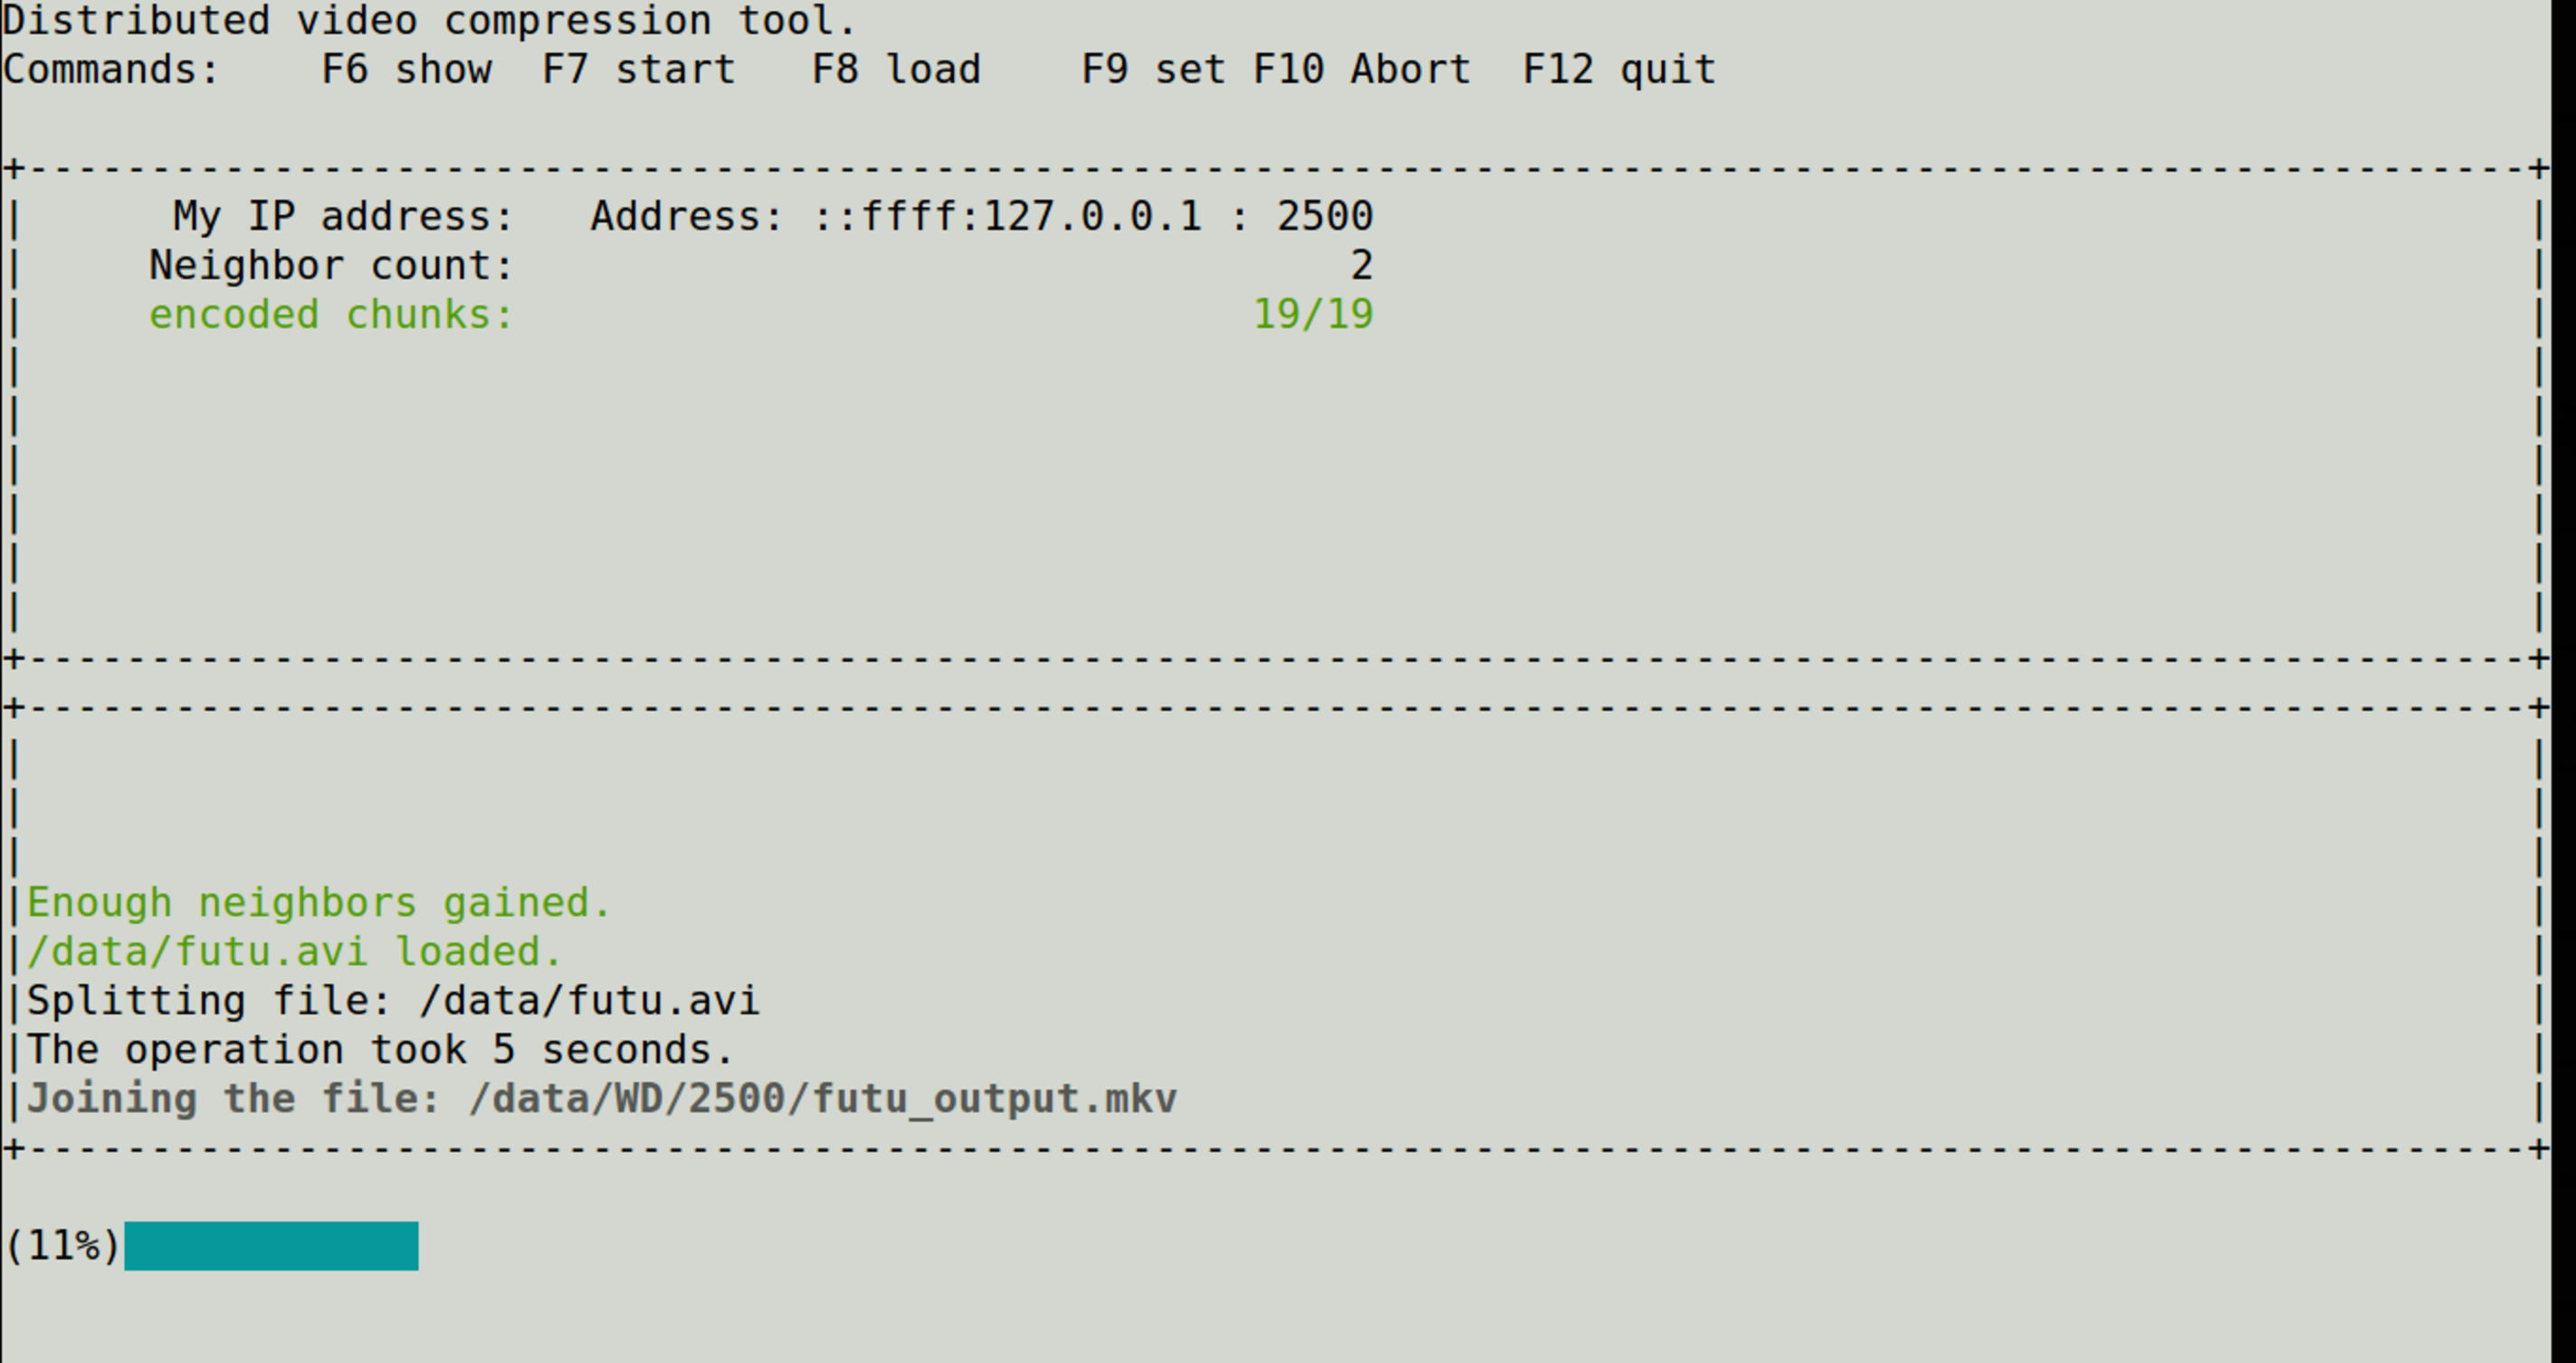
\includegraphics[scale=0.30]{./img/joining.pdf}
\caption{Joining the file.}
\end{center}
\end{figure}

To obtain more information about what is going on, the \textit{-d} option may be used which allows to specify level of debug messages that will be showed.
\section*{Appendix B - Attached software}
All the attached software can be found on the attached CD. It contains:
\begin{enumerate}
\item Sources of the framework, together with the installation script in the \textit{VideoCompression/} directory. This directory also contains the \textit{rapidjson} library and license agreements.
\item Documentation in the \textit{doc/} directory. To view this documentation, it is recommended to open the index.html file in your favorite html browser.
\item FFmpeg and x264 codec sources in the \textit{ffmpeg/} and \textit{x264/} directory.
\end{enumerate} 
\openright